\documentclass{beamer}
\usepackage[utf8]{inputenc}

\usetheme{Madrid}
  
\definecolor{cvut_navy}{HTML}{AA223C}
\definecolor{cvut_blue}{HTML}{636463}
\definecolor{cvut_gray}{HTML}{2977b9}

\setbeamercolor{section in toc}{fg=black,bg=white}
\setbeamercolor{alerted text}{fg=cvut_blue}
\setbeamercolor*{palette primary}{bg=cvut_navy,fg=gray!20!white}
\setbeamercolor*{palette secondary}{bg=cvut_blue,fg=white}
\setbeamercolor*{palette tertiary}{parent=palette primary}
\setbeamercolor*{palette quaternary}{fg=green,bg=gray!5!white}

\setbeamercolor*{sidebar}{fg=cvut_navy,bg=gray!15!white}


\setbeamercolor{titlelike}{parent=palette primary}
\setbeamercolor{frametitle}{parent=palette primary}

\setbeamercolor*{separation line}{}
\setbeamercolor*{fine separation line}{}

\usepackage[spanish]{babel}
\usepackage{eqnarray,amsmath}
\usepackage{amsfonts}
\usepackage{amssymb}
\usepackage{graphicx}
\usepackage{lmodern} % pro pismo tucne a zaroven kurziva
\usepackage{bm} % pro pismo tucne a zaroven kurziva
\usepackage{epstopdf}
\usepackage{changepage}
\usepackage{array,booktabs}
\usepackage{float}
\usepackage{subcaption}
\usepackage{hyperref}
\usepackage[T1]{fontenc}
\usepackage{calligra}




%====================================================
%========== DEFINITION OF AUTHORS ETC...=============
%====================================================
\author[Daniel Puente Ramírez]{Daniel Puente Ramírez}
\institute[]{Universidad de Burgos}
\title[Detección de baterías]{Detección de baterías mediante visión artificial}
\subtitle{Harware de Aplicación Específica}
\date{\today}

%====================================================
%========== BEGINNING OF DOCUMENT ===================
%====================================================
\begin{document}

\begin{frame}
	\titlepage
	\begin{center}
  		
\includegraphics[height=1.3cm]{img/Escudo-Apaisado}
		
\includegraphics[height=1.3cm]{img/Clarios}
	\end{center}
\end{frame}


\logo{
\includegraphics[height=1cm]{img/Escudo}}

\begin{frame}
\tableofcontents
\end{frame}


\begin{frame}{Planteamiento del problema}
\section{Planteamiento del problema}
Dado un vídeo de una cinta transportadora sobre la que discurren baterías de coche en su etapa final de fabricación. Se desea contabilizar el número de baterías que han pasado, independientemente de su tamaño, color, o la distancia a la que se debe montar la cámara.
\end{frame}

\begin{frame}{Planteamiento del problema}{Ejemplos de \textit{frames} - Vídeo 1}
\subsection{Ejemplo de \textit{frames}}
\begin{figure}
\centering
    \begin{subfigure}[t]{0.4\textwidth}
        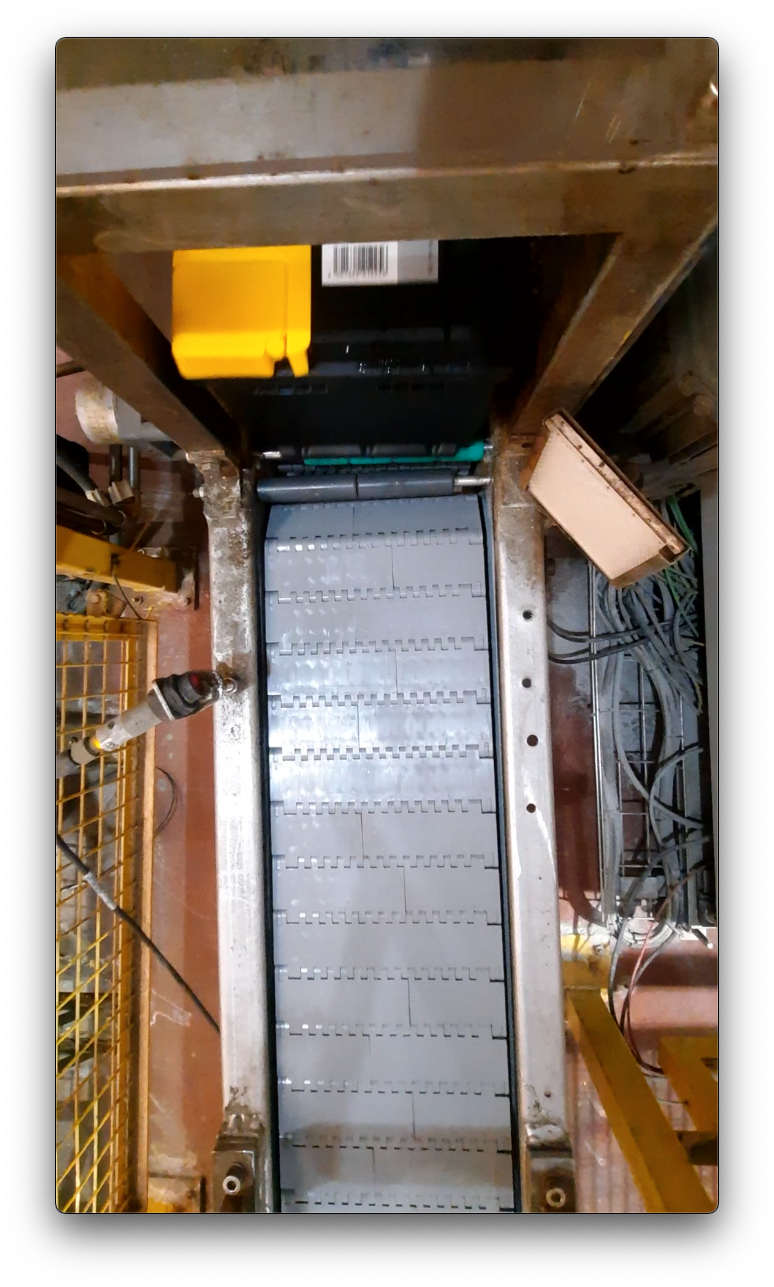
\includegraphics[width=\textwidth]{img/B1.png}
    \end{subfigure}
    \begin{subfigure}[b]{0.4\textwidth}
        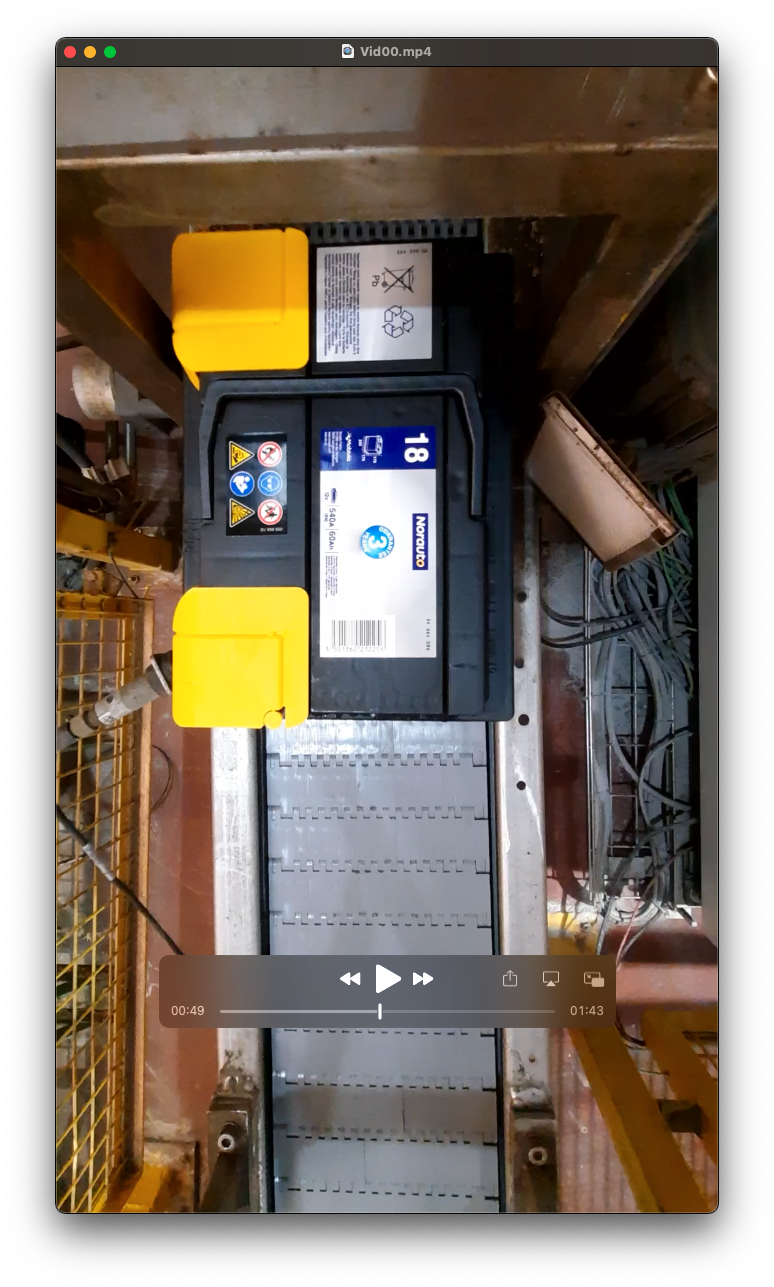
\includegraphics[width=\textwidth]{img/B2.png}
    \end{subfigure}
\end{figure}
\end{frame}

\begin{frame}{Planteamiento del problema}{Ejemplos de \textit{frames} - Vídeo 2}
\begin{figure}
\centering
    \begin{subfigure}[t]{0.4\textwidth}
        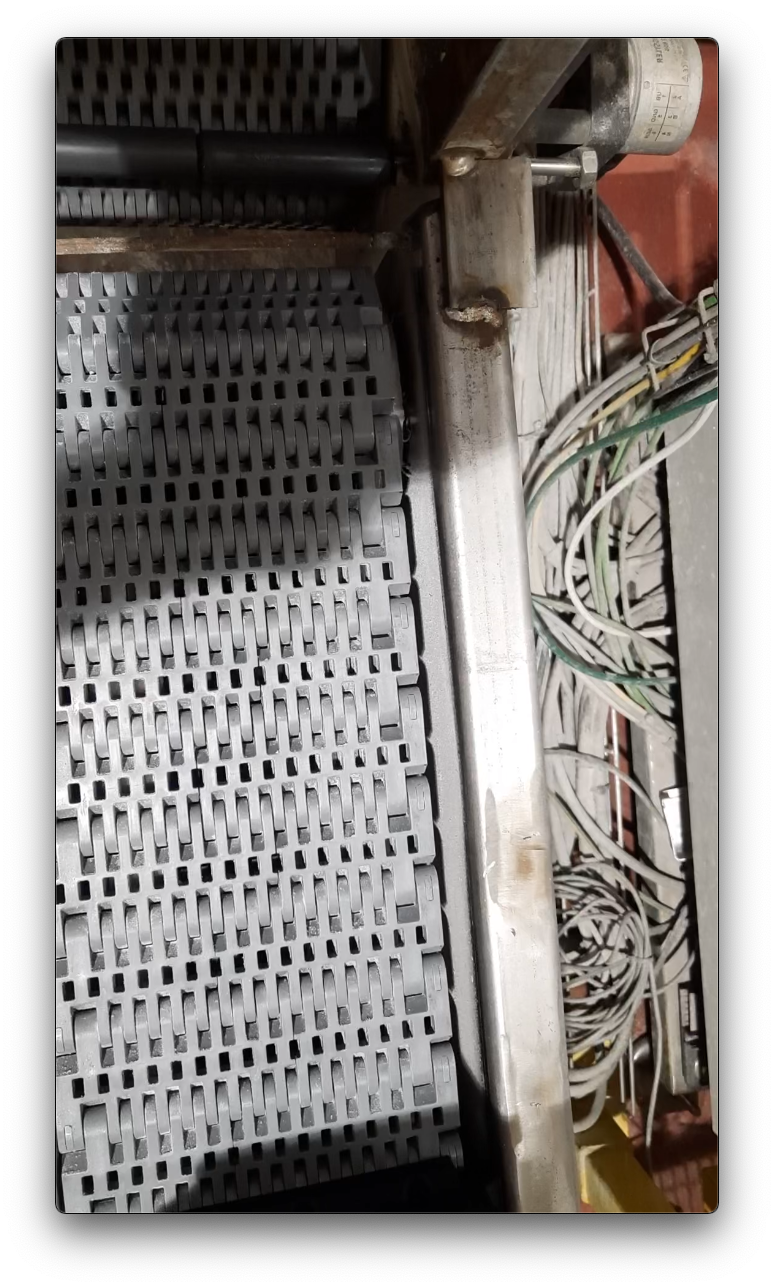
\includegraphics[width=\textwidth]{img/B3.png}
    \end{subfigure}
    \begin{subfigure}[b]{0.4\textwidth}
        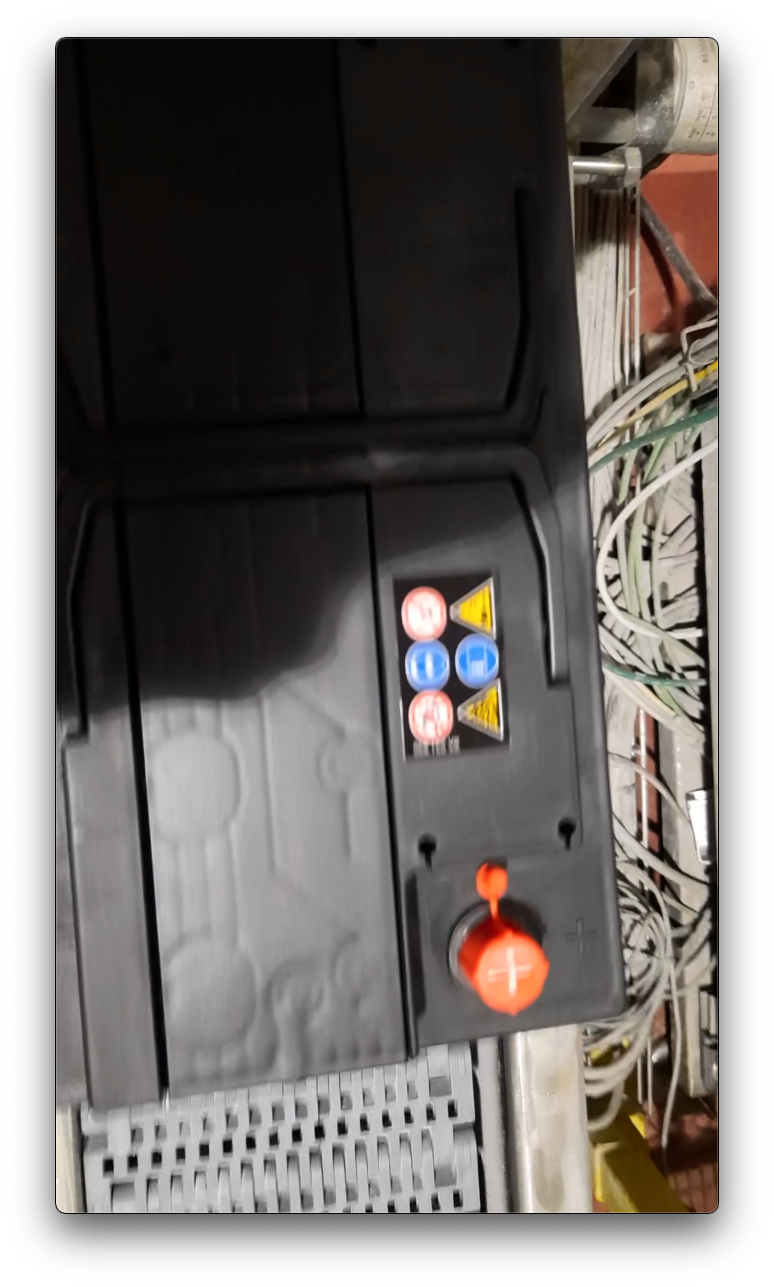
\includegraphics[width=\textwidth]{img/B4.png}
    \end{subfigure}
\end{figure}
\end{frame}

\begin{frame}{Planteamiento del problema}{Ejemplos de \textit{frames} - Vídeo 3}
\begin{figure}
\centering
    \begin{subfigure}[t]{0.4\textwidth}
        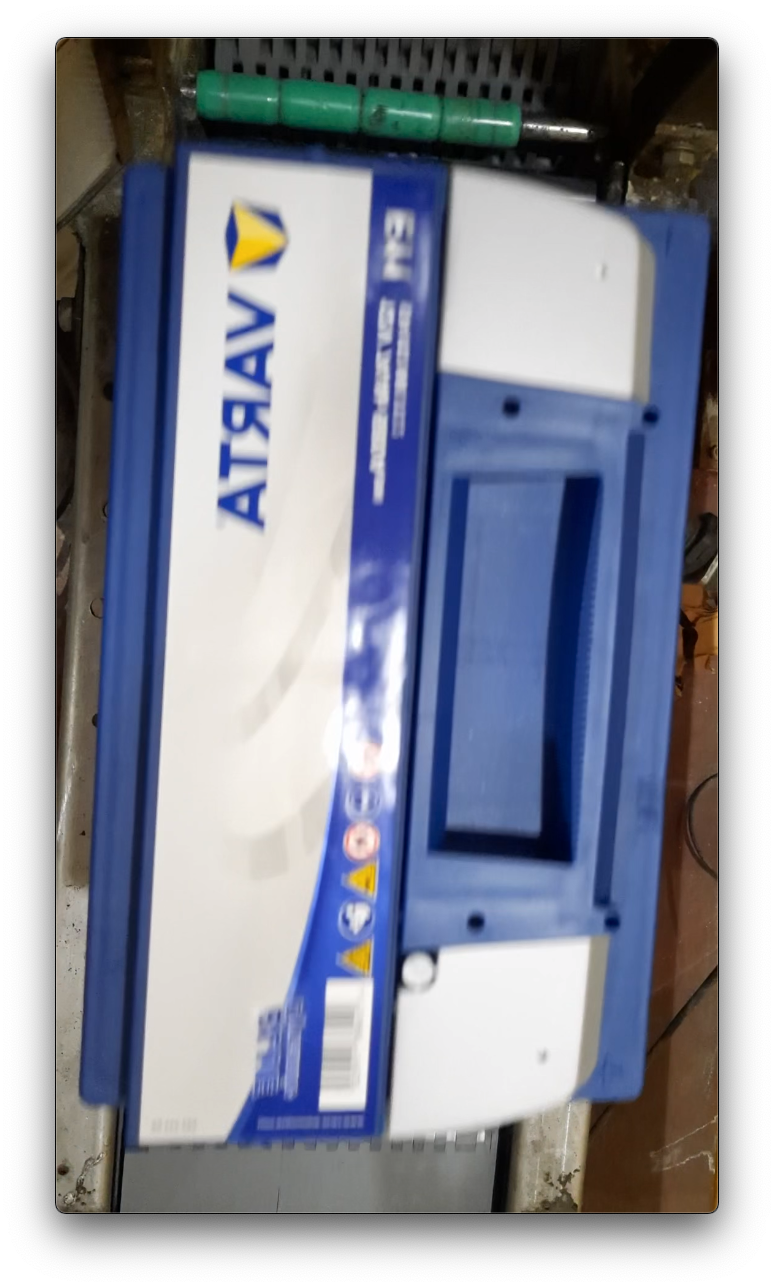
\includegraphics[width=\textwidth]{img/B5.png}
    \end{subfigure}
    \begin{subfigure}[b]{0.4\textwidth}
        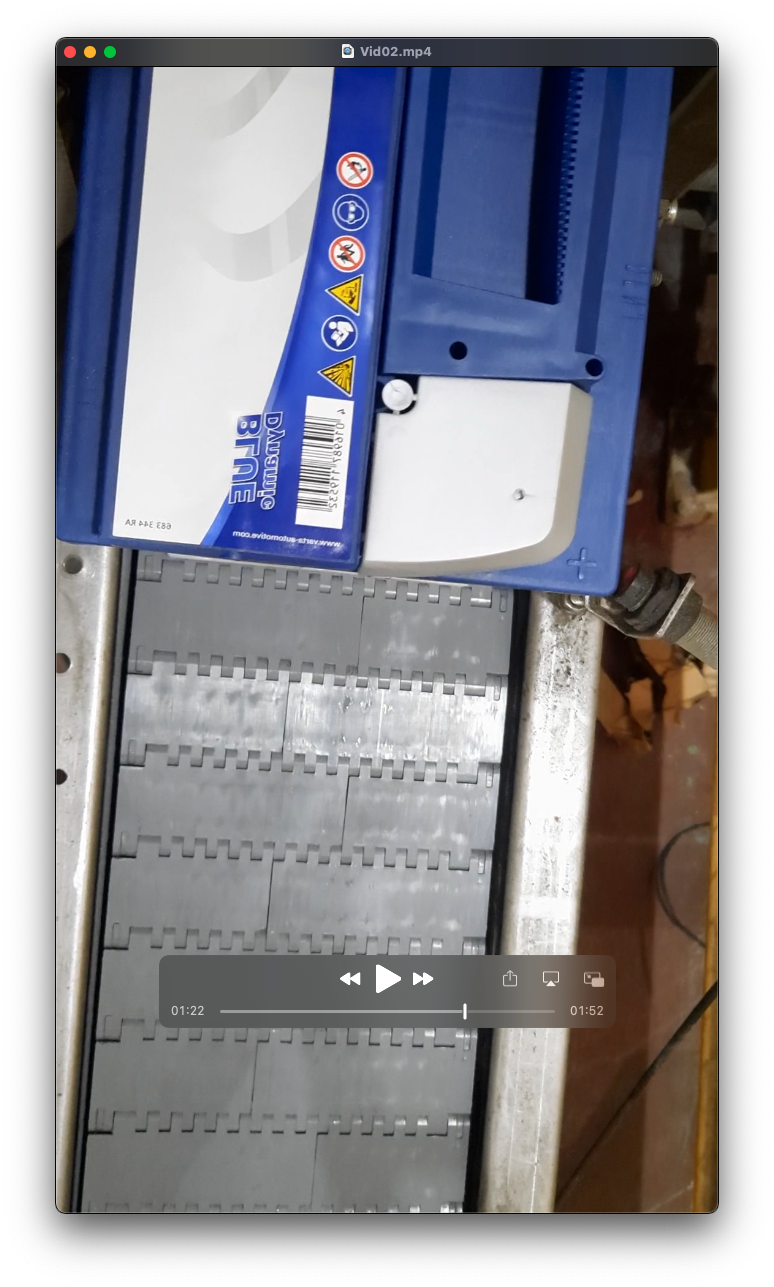
\includegraphics[width=\textwidth]{img/B6.png}
    \end{subfigure}
\end{figure}
\end{frame}

\begin{frame}{Solución propuesta}{Reconocimiento del fondo}
\section{Solución propuesta}
\subsection{Reconocimiento del fondo}

Detección del fondo de cada vídeo. Detección mediante \textbf{Background subtraction} $\rightarrow$ \textbf{Media acumulativa}.

\begin{align*}
	B(t)  = \left(1-\alpha\right) \times B\left(t-1\right) + \alpha \times I\left(t-1\right) \\
	F(t) = \left| I(t) - B(t)\right| > \text{umbral} \\	
	\alpha = 0.05 \rightarrow \text{Parámetro de aprendizaje}
\end{align*}

El fondo no es calculado de manera dinámica ya que la práctica simula una instalación fija de la cual se conoce posición, ángulo, etcétera.
\end{frame}

\begin{frame}{Solución propuesta}{Fondos reconocidos}
\subsection{Tratamiento de la imagen}
\begin{figure}
\centering
    \begin{subfigure}[t]{0.3\textwidth}
        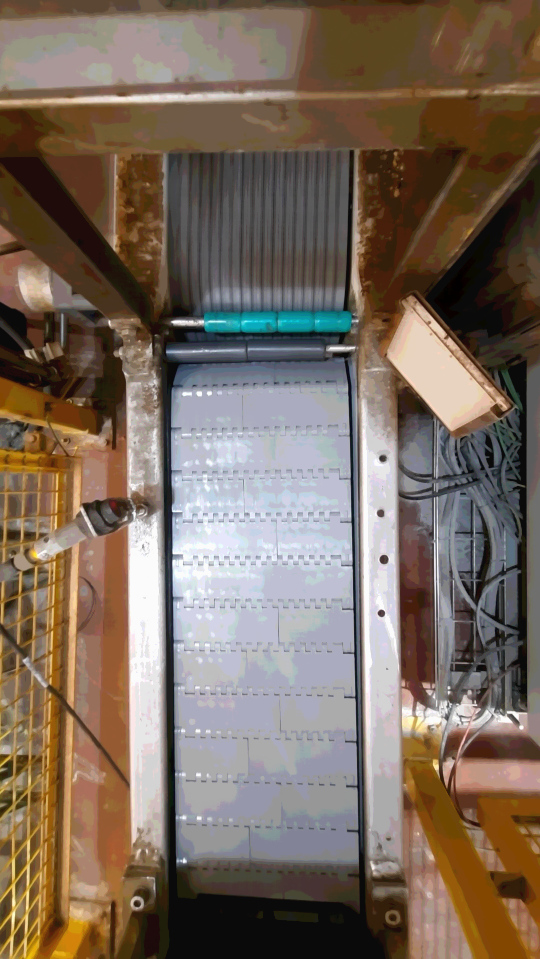
\includegraphics[width=\textwidth]{img/F1.png}
    \end{subfigure}
    \begin{subfigure}[b]{0.3\textwidth}
        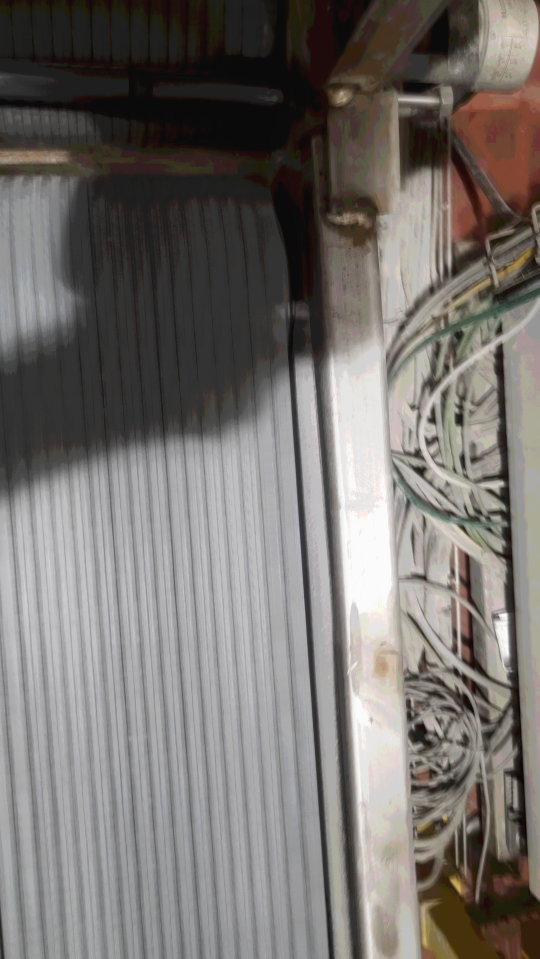
\includegraphics[width=\textwidth]{img/F2.png}
    \end{subfigure}
    \begin{subfigure}[b]{0.3\textwidth}
        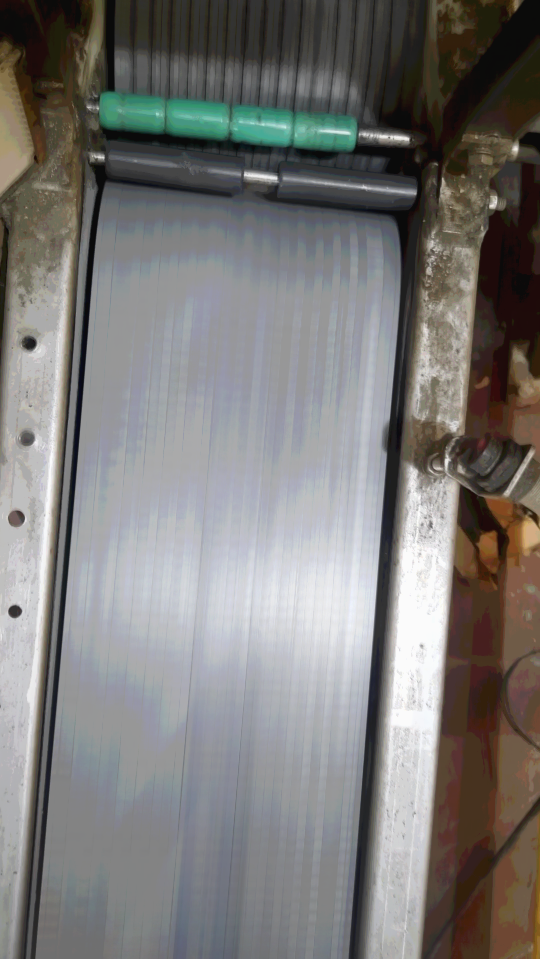
\includegraphics[width=\textwidth]{img/F3.png}
    \end{subfigure}
\end{figure}
Fondos de los vídeos $\lbrace Vid00, Vid01, Vid02 \rbrace$ respectivamente.
\end{frame}

\begin{frame}{Reconocimiento de baterías}{Modificación de los \textit{frames}}
\centering
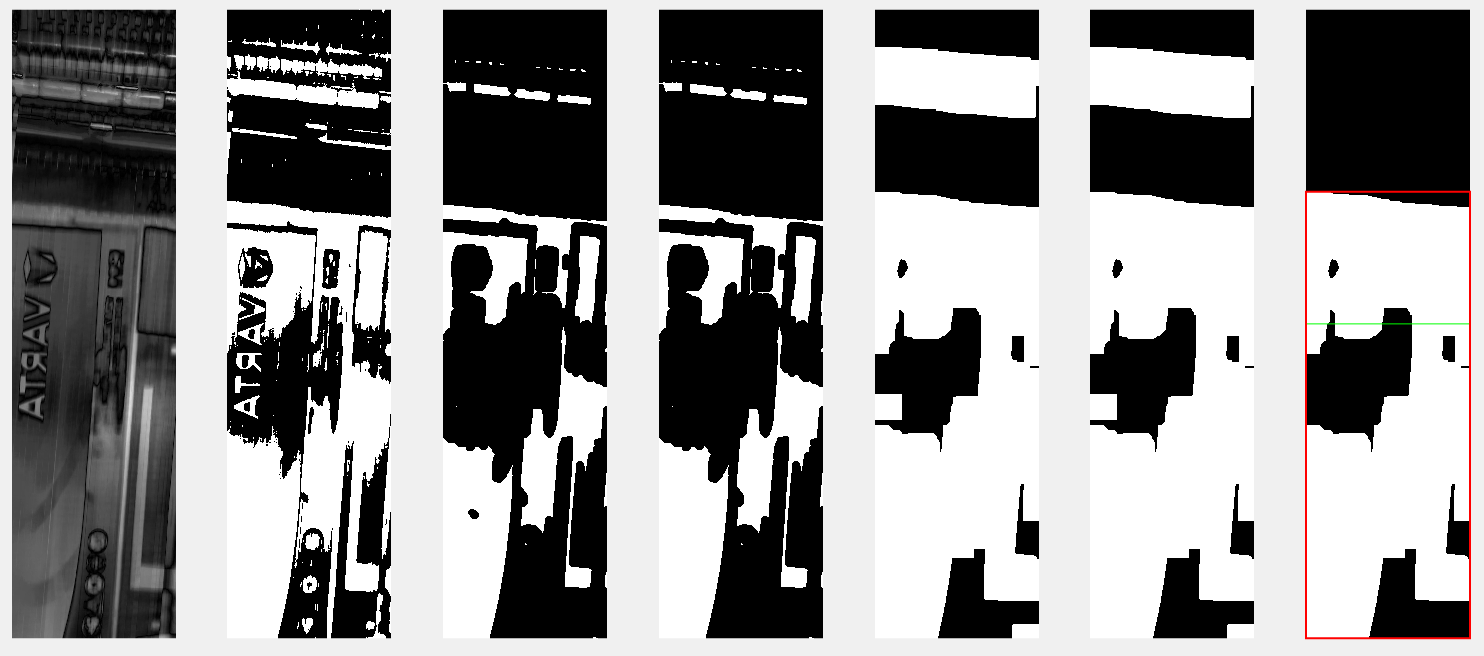
\includegraphics[width=0.95\paperwidth, height=0.8\paperheight]{img/T1}%
\end{frame}

\begin{frame}{Reconocimiento de baterías}{Modificación de los \textit{frames}}
\centering
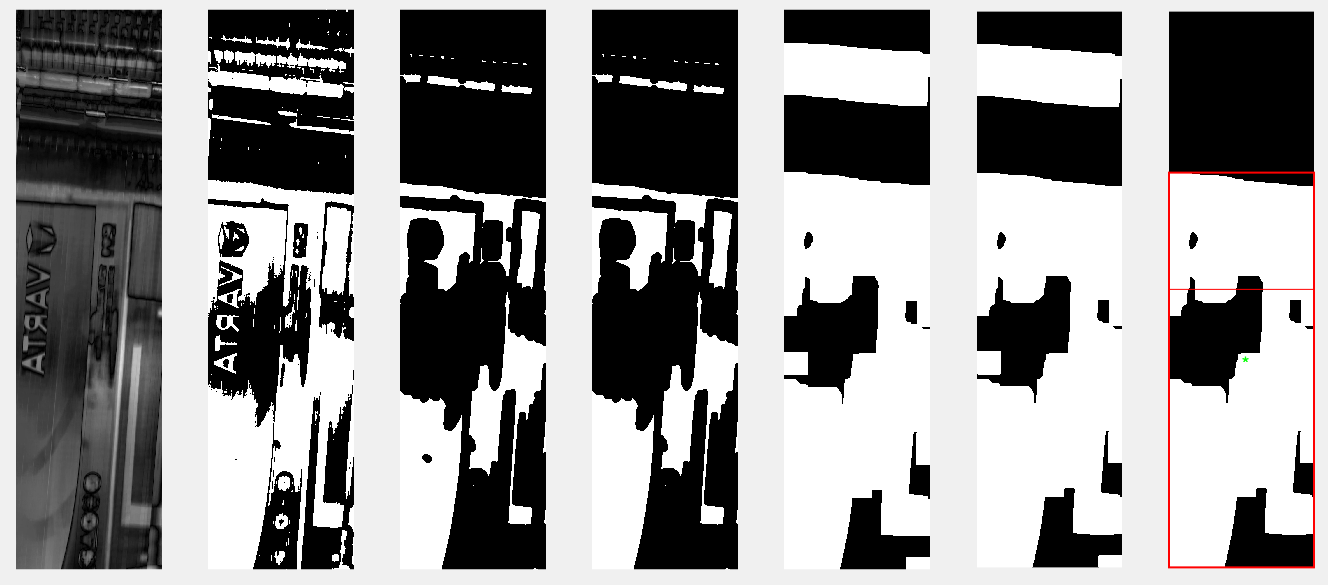
\includegraphics[width=0.95\paperwidth, height=0.8\paperheight]{img/T2}%
\end{frame}

\begin{frame}{Reconocimiento de baterías}{Modificación de los \textit{frames}}
\centering
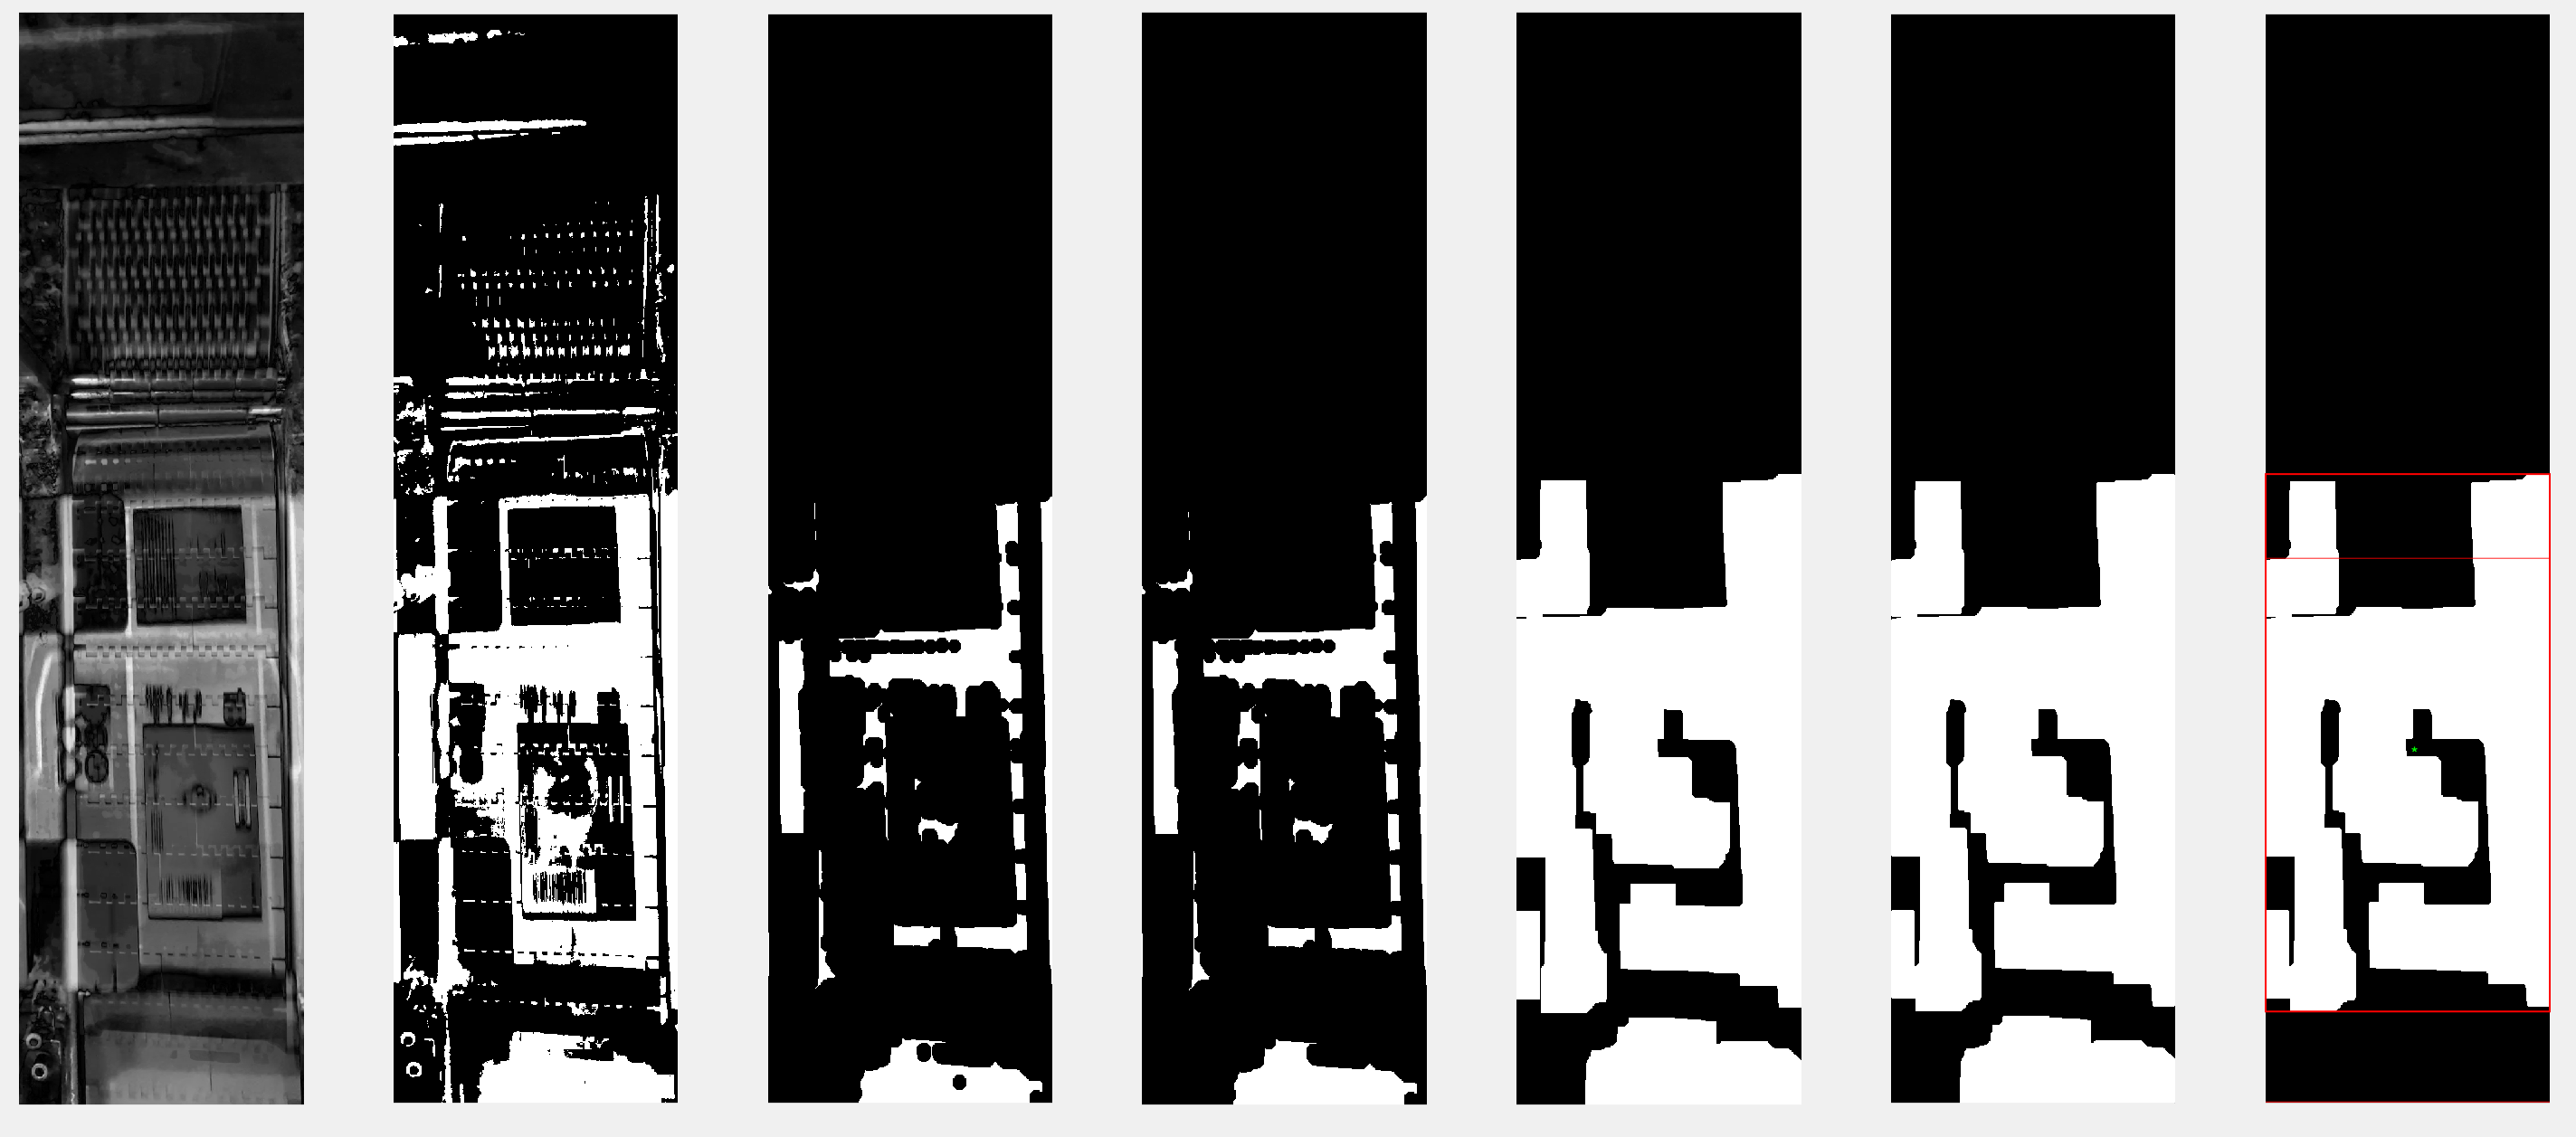
\includegraphics[width=0.95\paperwidth, height=0.8\paperheight]{img/T3}%
\end{frame}

\begin{frame}{Reconocimiento de baterías}{Visualización sobre el \textit{frame} original}
\subsection{Aplicación sobre la imagen}
\begin{figure}
\centering
    \begin{subfigure}[t]{0.4\textwidth}
        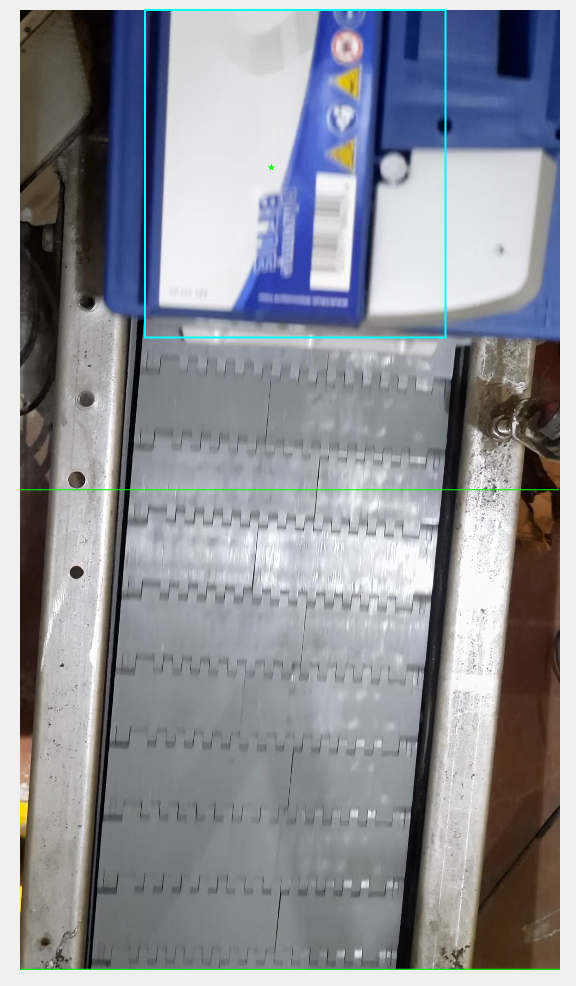
\includegraphics[width=\textwidth]{img/P1.png}
    \end{subfigure}
    \begin{subfigure}[b]{0.4\textwidth}
        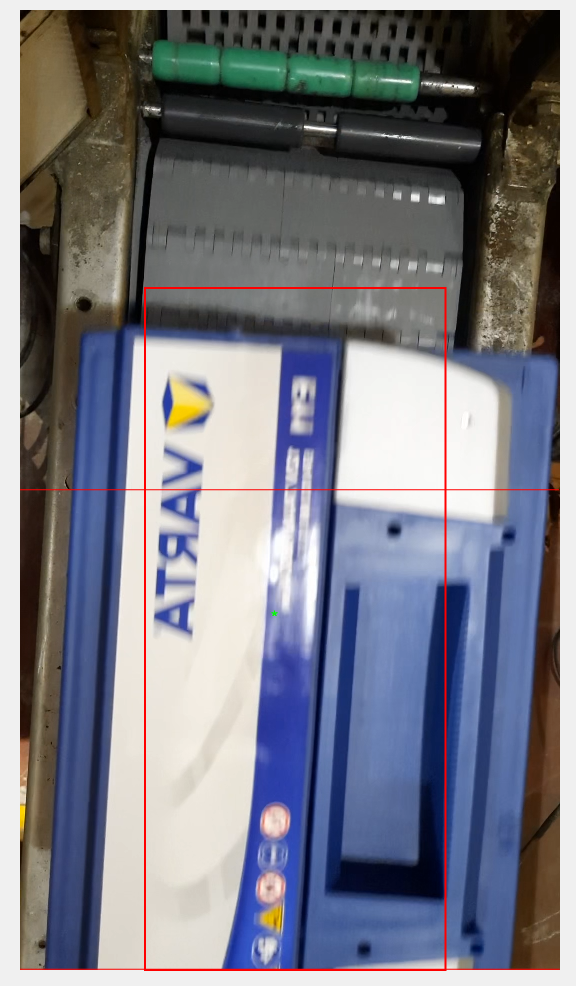
\includegraphics[width=\textwidth]{img/P2.png}
    \end{subfigure}
\end{figure}
\end{frame}

\begin{frame}{Salida producida}{Visualización de la salida producida por parte de los 3 vídeos.}
\subsection{Resultados}
\begin{figure}
\begin{center}
\begin{subfigure}[t]{0.3\textwidth}
        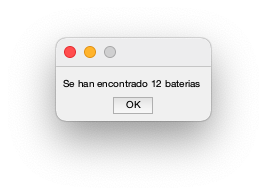
\includegraphics[width=\textwidth]{img/S0.png}
        \caption{Vídeo 0}
    \end{subfigure}
    \begin{subfigure}[b]{0.3\textwidth}
        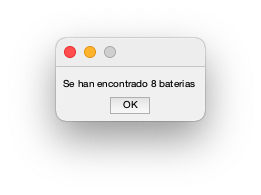
\includegraphics[width=\textwidth]{img/S1.png}
        \caption{Vídeo 1}
    \end{subfigure}
    \begin{subfigure}[b]{0.3\textwidth}
        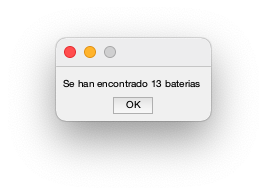
\includegraphics[width=\textwidth]{img/S2.png}
        \caption{Vídeo 2}
    \end{subfigure}
\end{center}
    
\end{figure}
\end{frame}

\begin{frame}
    \begin{center}
        \Huge\calligra ¿Alguna pregunta?
    \end{center}
\end{frame}
\end{document}

% =============================================================
% =========================== END =============================
% =============================================================